\documentclass[12pt]{article}
\usepackage{amsmath}
\usepackage{amsfonts}
\usepackage{url}
\usepackage{float}
\usepackage{multicol}
\usepackage{chemformula}
\usepackage{hyperref}
\hypersetup{
	colorlinks=true,
	linkcolor=blue,
	filecolor=magenta,      
	urlcolor=blue,
	citecolor=blue
}
\usepackage{graphicx}
\usepackage{subcaption}
\usepackage{url}
\usepackage{siunitx}
\usepackage{listings}
\usepackage{color} %red, green, blue, yellow, cyan, magenta, black, white
\definecolor{mygreen}{RGB}{28,172,0} % color values Red, Green, Blue
\definecolor{mylilas}{RGB}{170,55,241}
\setlength{\oddsidemargin}{0in}
\setlength{\evensidemargin}{0in}
\setlength{\textheight}{9in}
\setlength{\textwidth}{6.5in}
\setlength{\topmargin}{-0.5in}
\usepackage[backend=biber,sorting=none,style=nature]{biblatex}
\addbibresource{biblio.bib}

\DeclareSIUnit\atm{atm}

\title{\bf Assignment 2 \\[2ex] 
	\rm\normalsize Electronic Structure Theory}
\date{\today}
\author{\bf Declan Mathews [s1610357][B103565]}

\begin{document}
	\maketitle
	
\section*{Silicon Elastic Properties}
\subsection*{Rhombohedral lattice input}
\lstinputlisting[firstline=8, lastline=14]{lattice-data/si.scf-ibrav5-van.in}
\lstinputlisting[firstline=23, lastline=31]{lattice-data/si.scf-ibrav5-van.in}

\subsection*{Simple cubic lattice input}
\lstinputlisting[firstline=8, lastline=13]{lattice-data/si.scf-ibrav1-van.in}
\lstinputlisting[firstline=22, lastline=30]{lattice-data/si.scf-ibrav1-van.in}

\subsection*{Tetragonal lattice input}
\lstinputlisting[firstline=8, lastline=14]{lattice-data/si.scf-ibrav6-van.in}
\lstinputlisting[firstline=23, lastline=31]{lattice-data/si.scf-ibrav6-van.in}

\subsection*{Lattice check results}
\begin{table}[h!!!!]
	\centering
\begin{tabular}{c|c|cll}
	\cline{2-2}
	& Total energy (Ry) &  &  &  \\ \cline{1-2}
	\multicolumn{1}{|l|}{Simple Cubic} & -76.76877937      &  &  &  \\ \cline{1-2}
	\multicolumn{1}{|l|}{Rhombohedral} & -76.76877936      &  &  &  \\ \cline{1-2}
	\multicolumn{1}{|l|}{Tetragonal}   & -76.76877937      &  &  &  \\ \cline{1-2}
\end{tabular}
\caption{The SCF calculation energy results for the varying methods of initial structure input for Silicon.}
\label{tab:lattice-check}
\end{table}

\noindent Using the inputs stated above, the SCF results in Table \ref{tab:lattice-check} were gathered. Clearly the different lattices all give an almost identical result, with a small difference likely due to k-point sampling methods.

\subsection*{Silicon elastic constants}

\noindent SCF calculations were then performed on the tetragonal lattice of Silicon. This was done for a varying $c/a$ ratio, which corresponds to a finite strain $\epsilon_{33}$. The stress tensor components $\sigma_{11}$ and $\sigma_{33}$ were plotted against the ratio as shown in Figure \ref{fig:si-elastic}. A straight line fit was performed to find the gradient, the negative of which provided the $c_{11}$ and $c_{13}$ elastic constants of Silicon, as stated in Table \ref{tab:si-elastic}. Experimental values\footnote{\label{foot: Si}http://sense.fas.sfu.ca/internal/Si\_elastic.pdf} give $c_{11} = $ \num{1.6564e11} Pa, which is equal to $165.64$ GPa, and $c_{13} = $ \num{0.6394e11} Pa, equal to $63.94$ GPa. These are in good agreement with the gathered data.

\begin{figure}[h!!!!!]
\centering
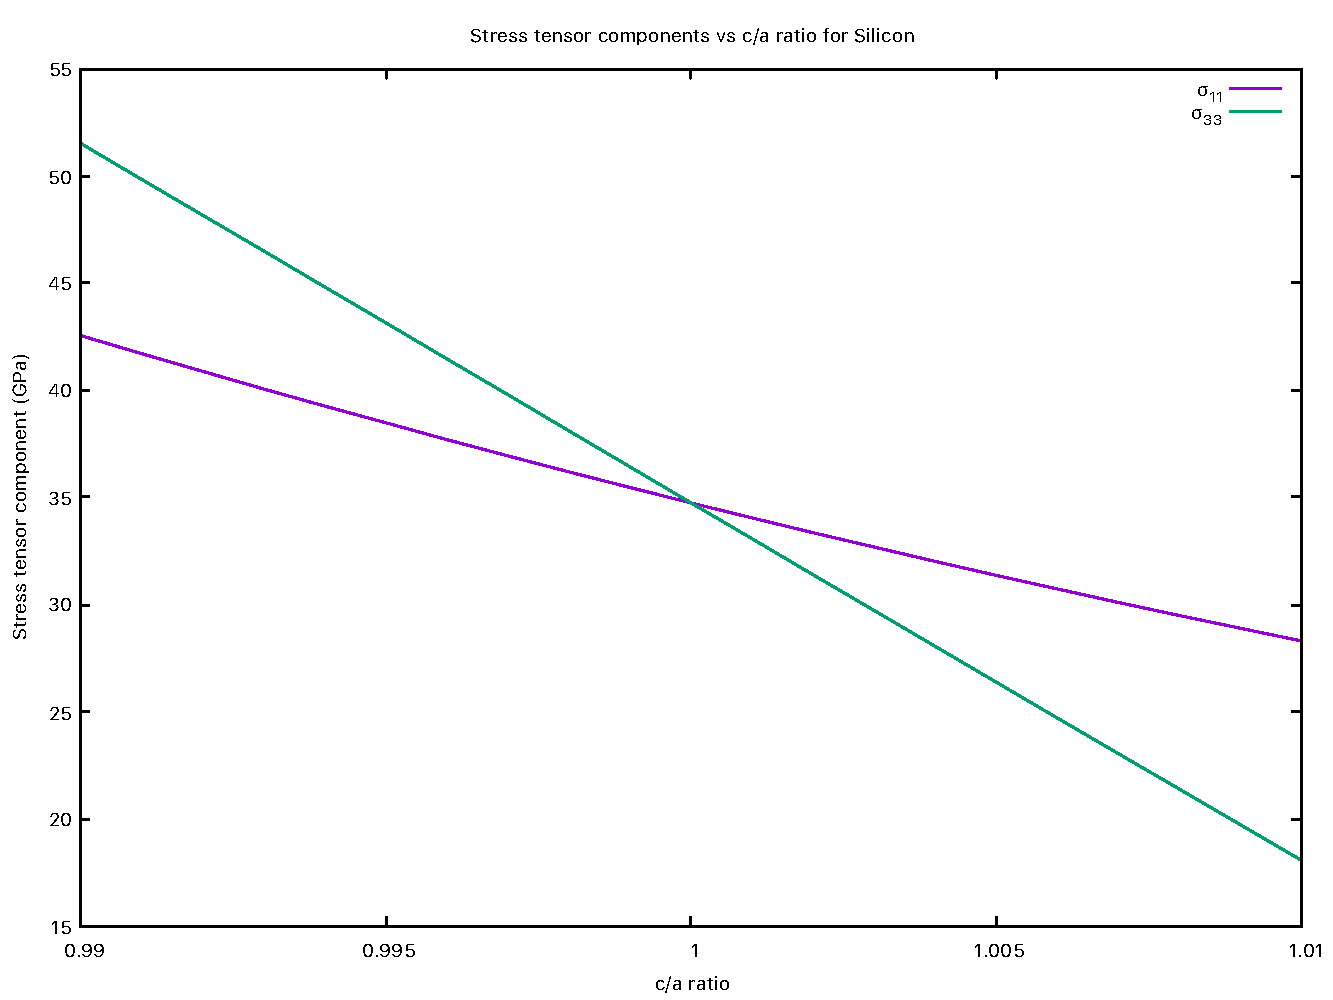
\includegraphics[width=12cm]{elastic-data/si-elastic-plot.pdf}
\caption{The variation in different stress tensor components of Silicon with the c/a ratio. This c/a ratio is analgous to the strain rate $\epsilon_{33}$ and so the elastic constants can be found via the gradient.}
\label{fig:si-elastic}
\end{figure}

\begin{table}[h!!!!!]
	\centering
	\begin{tabular}{l|c|c|c|}
		\cline{2-4}
		\multicolumn{1}{c|}{}           & Experiment (GPa) & Fit (GPa)         & Error (GPa)              \\ \hline
		\multicolumn{1}{|l|}{c$_{11}$} & 165.64 & 167.453             & 0.066 (0.039 \%)         \\ \hline
		\multicolumn{1}{|l|}{c$_{13}$} & 63.94 & 71.187              & 0.846 (1.189 \%)         \\ \hline
	\end{tabular}
\caption{A table showing the results of the derived elastic constants of Silicon from the data in Figure \ref{fig:si-elastic} and the experimental values from footnote \ref{foot: Si}.}
\label{tab:si-elastic}
\end{table}


\clearpage
\section*{Electronic Density of States and Band Structures}

By fixing the Gaussian smearing at a small value and varying the NSCF k-point grid, the results for the density of states of Quartz, $\alpha$- and $\beta$-tin shown in Figure \ref{fig:k-vary} were obtained. For quartz and $\alpha$-tin the results begin to converge as k is increased. However, $\beta$-tin does not show this same convergence, likely due to its more complex structure requiring a very dense grid to model more correctly.

\begin{figure}[h!!!!!]
	\centering
	\begin{subfigure}[t]{0.5\textwidth}
		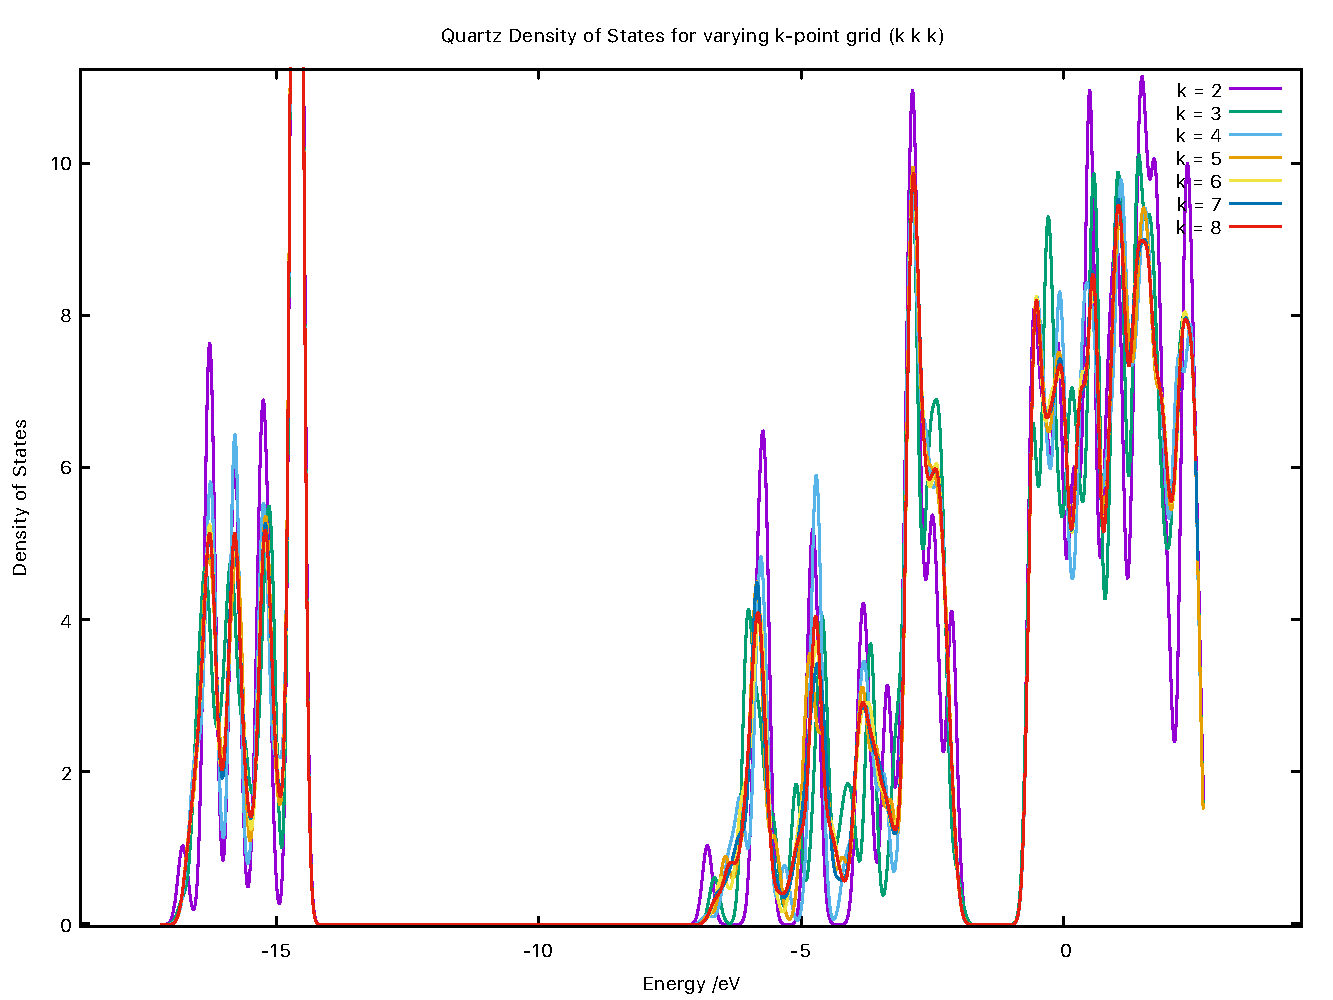
\includegraphics[width=8.2cm]{quartz-dos-data/quartz-k-vary-dos.pdf}
		\subcaption{Here the Gaussian smearing is at 0.010}
		\label{fig:quartz-k-dos}
	\end{subfigure}%
	\begin{subfigure}[t]{0.5\textwidth}
		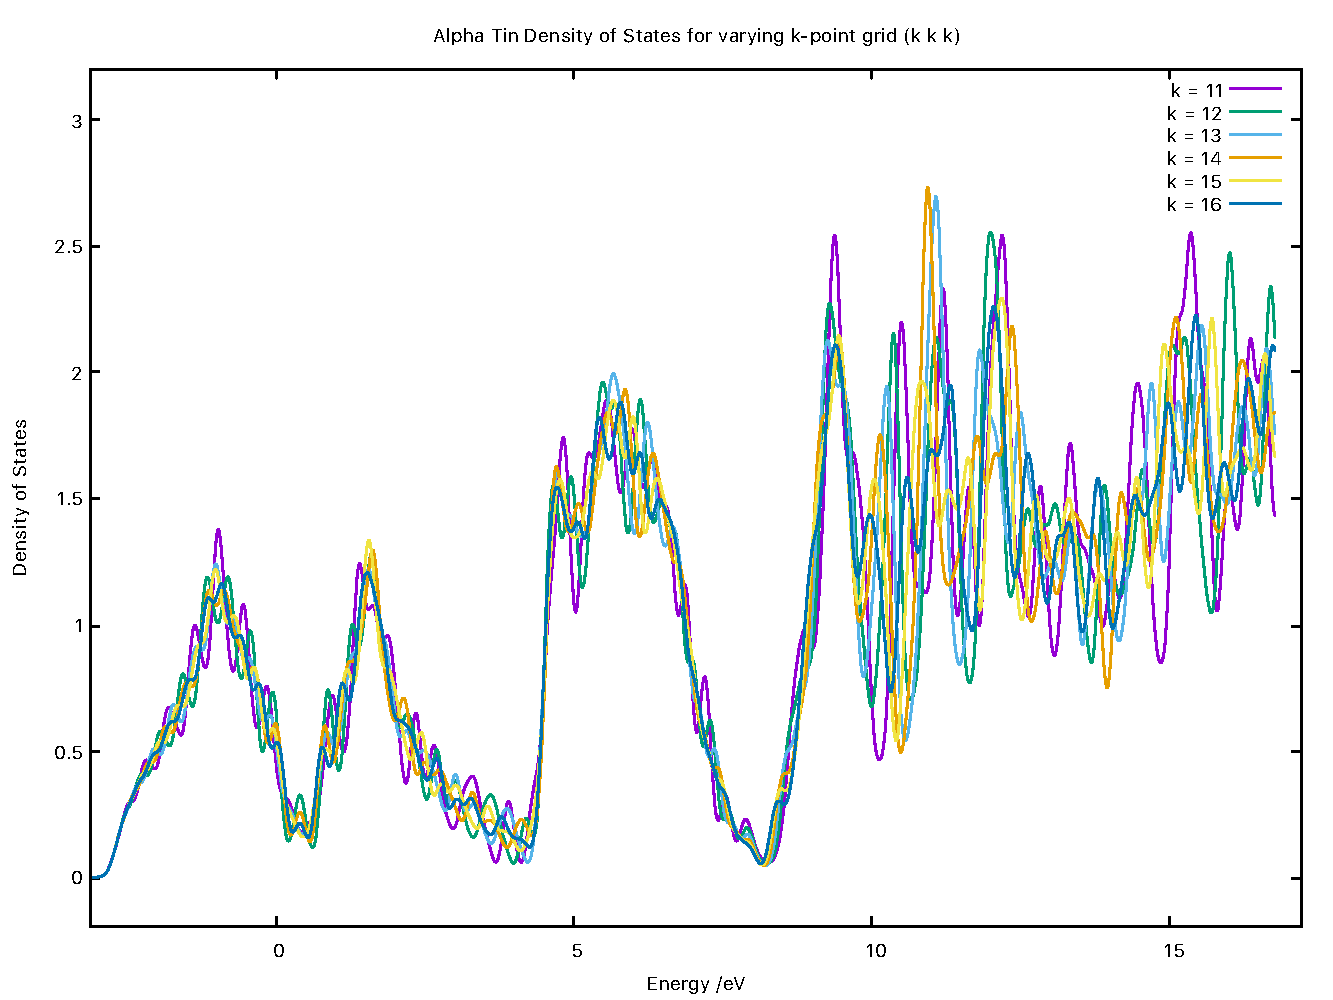
\includegraphics[width=8.2cm]{alpha-dos-data/alpha-k-vary-dos.pdf}
		\subcaption{Here the Gaussian smearing is at 0.010}
		\label{fig:alpha-k-dos}
	\end{subfigure}%
	\\
	\begin{subfigure}[t]{0.5\textwidth}
		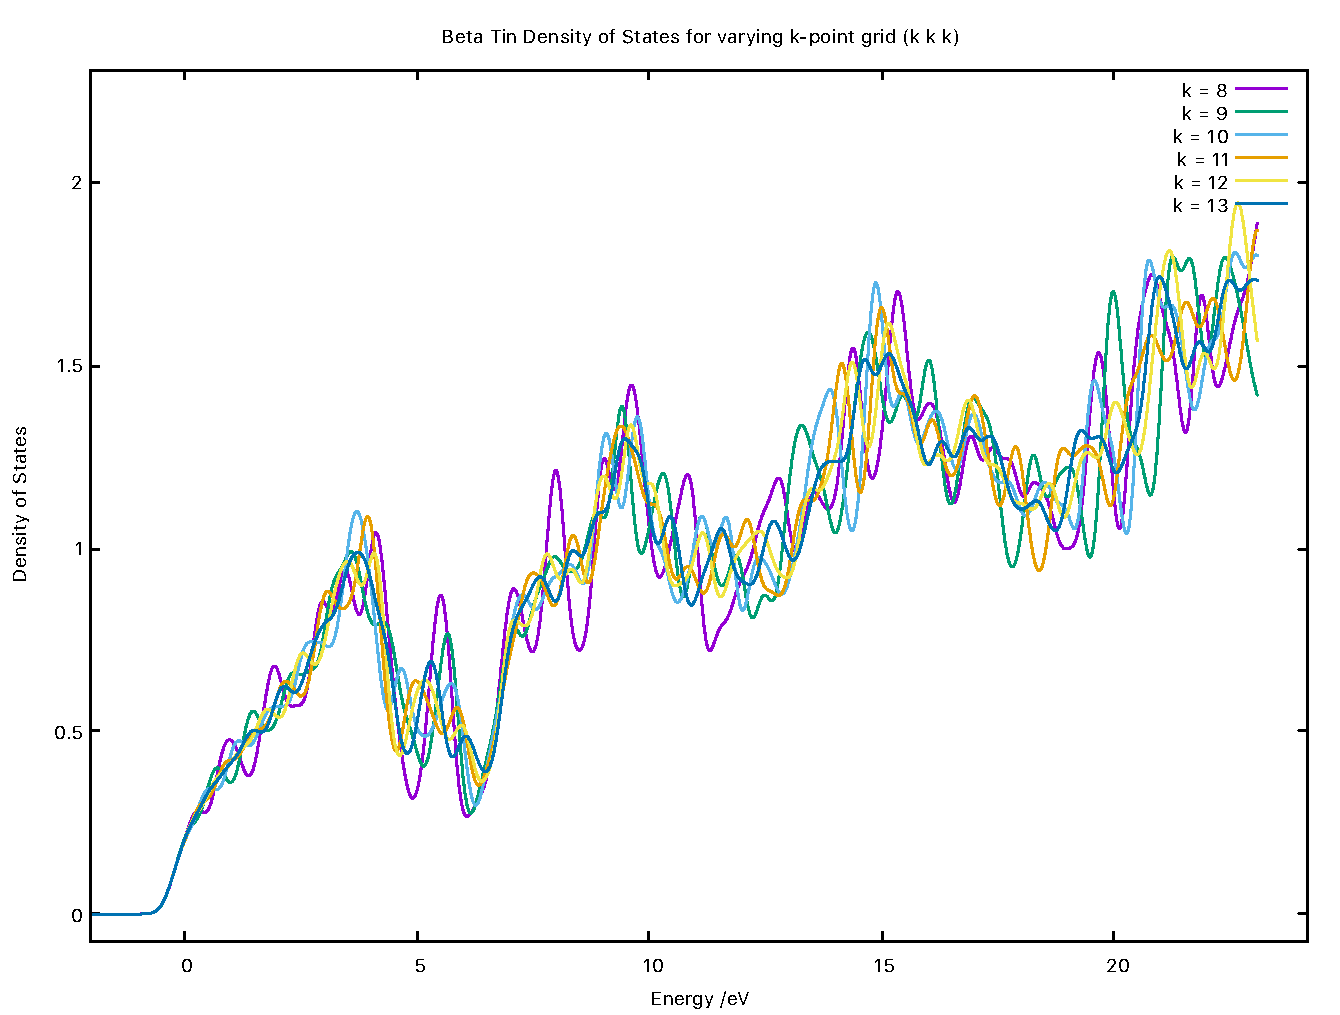
\includegraphics[width=8.2cm]{beta-dos-data/beta-k-vary-dos.pdf}
		\subcaption{Here the Gaussian smearing is at 0.020}
		\label{fig:beta-k-dos}
	\end{subfigure}
	\caption{The density fo states plotted with a varying k-point grid in the NSCF step for Quartz (a), $\alpha$- (b) and $\beta$-tin (c).}
	\label{fig:k-vary}
\end{figure}

\noindent Figure \ref{fig:gs-vary} shows the results for density of states when the k-point grid is held constant and the Gaussian smearing value is changed. This data all follows the same trend of converging towards a defined state for lower smearing values. This is expected as this merely an interpreting method of the data obtained from the calculations and not calculating the data at different points like when varying the k-point grid. Clearly a smaller value will converge more accurately to the calculated points but at increasing computational cost. Due to this the $\beta$-tin data was sampled over a smaller range as these computations were quite expensive due to its complex structure.

\begin{figure}[h!!!!!]
	\centering
	\begin{subfigure}[t]{0.5\textwidth}
		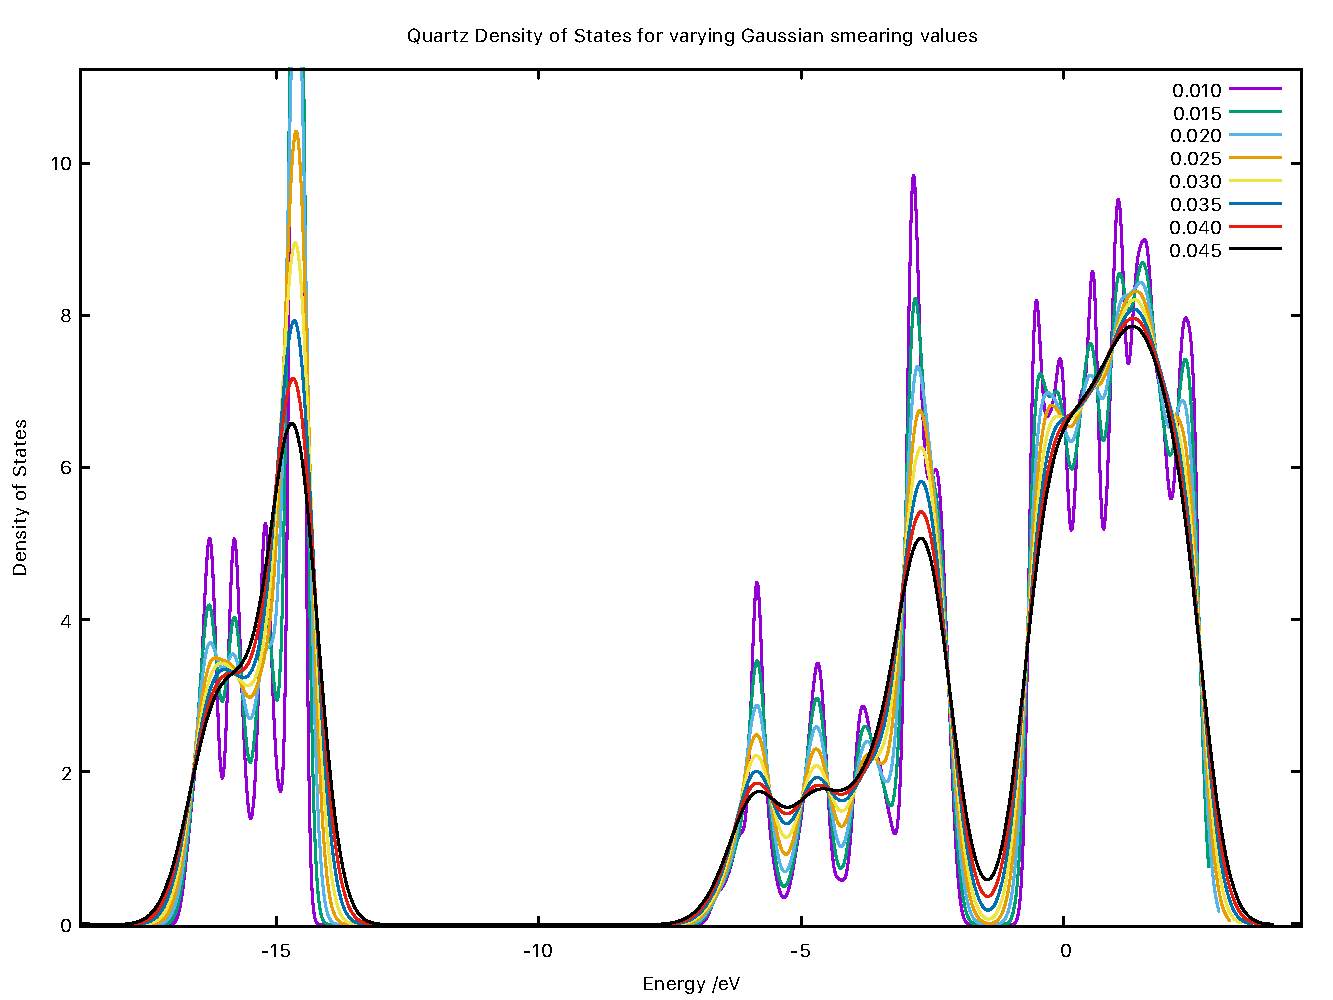
\includegraphics[width=8.2cm]{quartz-dos-data/quartz-smear-vary-dos.pdf}
		\subcaption{Here the k-point grid (k k k) has k = 7}
		\label{fig:quartz-gs-dos}
	\end{subfigure}%
	\begin{subfigure}[t]{0.5\textwidth}
		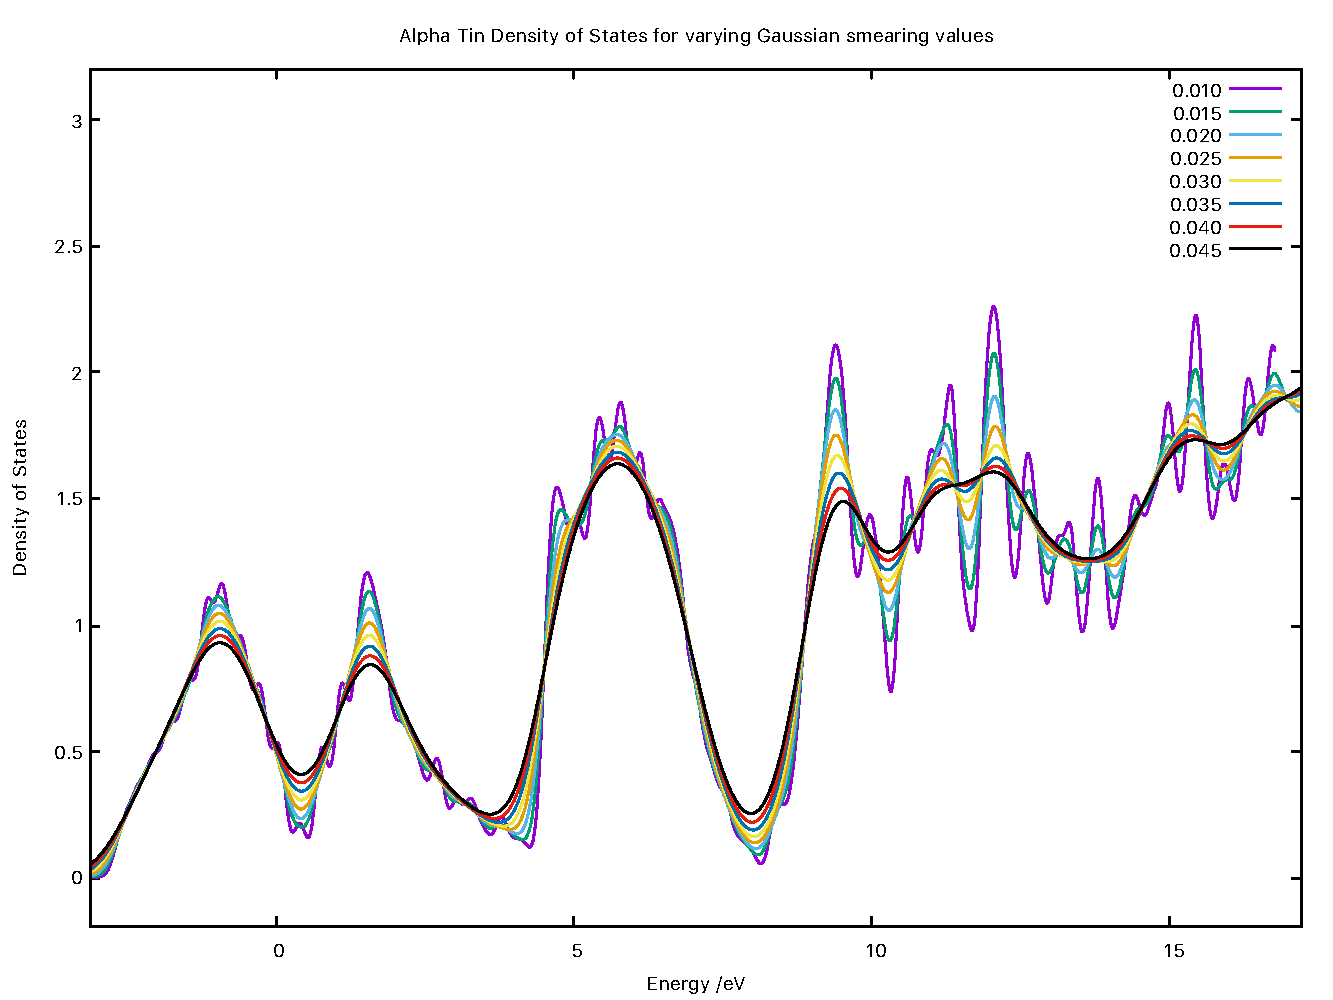
\includegraphics[width=8.2cm]{alpha-dos-data/alpha-smear-vary-dos.pdf}
		\subcaption{Here the k-point grid (k k k) has k = 16}
		\label{fig:alpha-gs-dos}
	\end{subfigure}%
	\\
	\begin{subfigure}[t]{0.5\textwidth}
		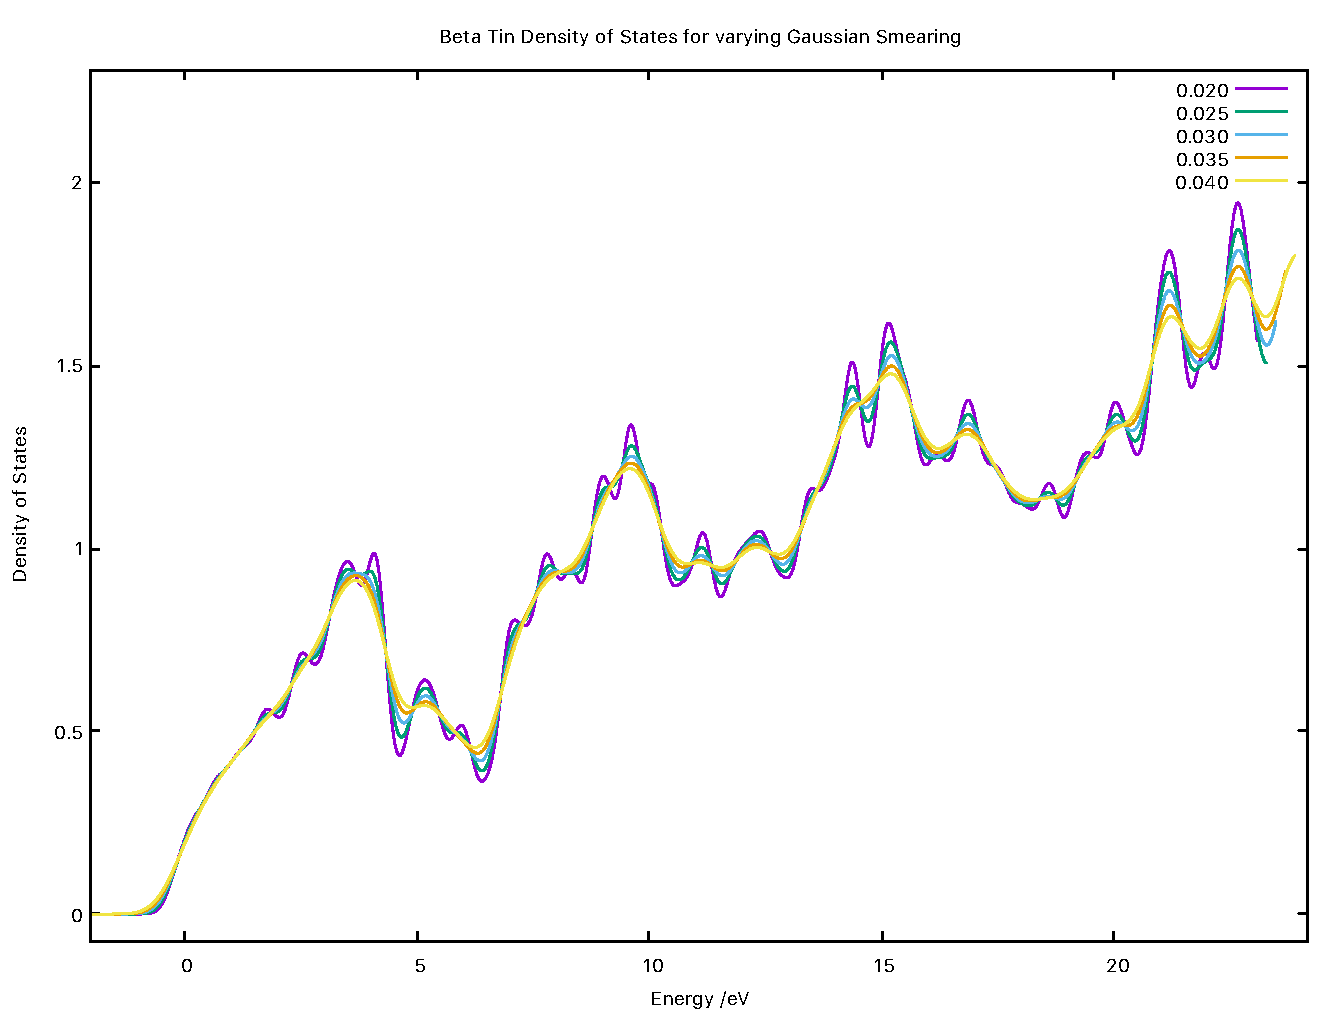
\includegraphics[width=8.2cm]{beta-dos-data/beta-smear-vary-dos.pdf}
		\subcaption{Here the k-point grid (k k k) has k = 12}
		\label{fig:beta-gs-dos}
	\end{subfigure}
	\caption{The density of states plotted with a Gaussian smearing value for Quartz (a), $\alpha$- (b) and $\beta$-tin (c). Note that due to time issues $\beta$-tin was ran over a smaller sample.}
	\label{fig:gs-vary}
\end{figure}

\noindent Another option instead of Gaussian smearing is tetrahedron interpolation. The results for a fixed k-point grid plot comparing the tetrahdron and smearing methods is shown in Figure \ref{fig:m-vary}. This data illustrates how the choice of interpolation can lead to far noiser and less clear data like for quartz, or for much clearer and less noisy data like for $\alpha$-tin. This choice is very system dependent and can also depend on the k-point grid choice.

\begin{figure}[h!!!!!]
	\centering
	\begin{subfigure}[t]{0.5\textwidth}
		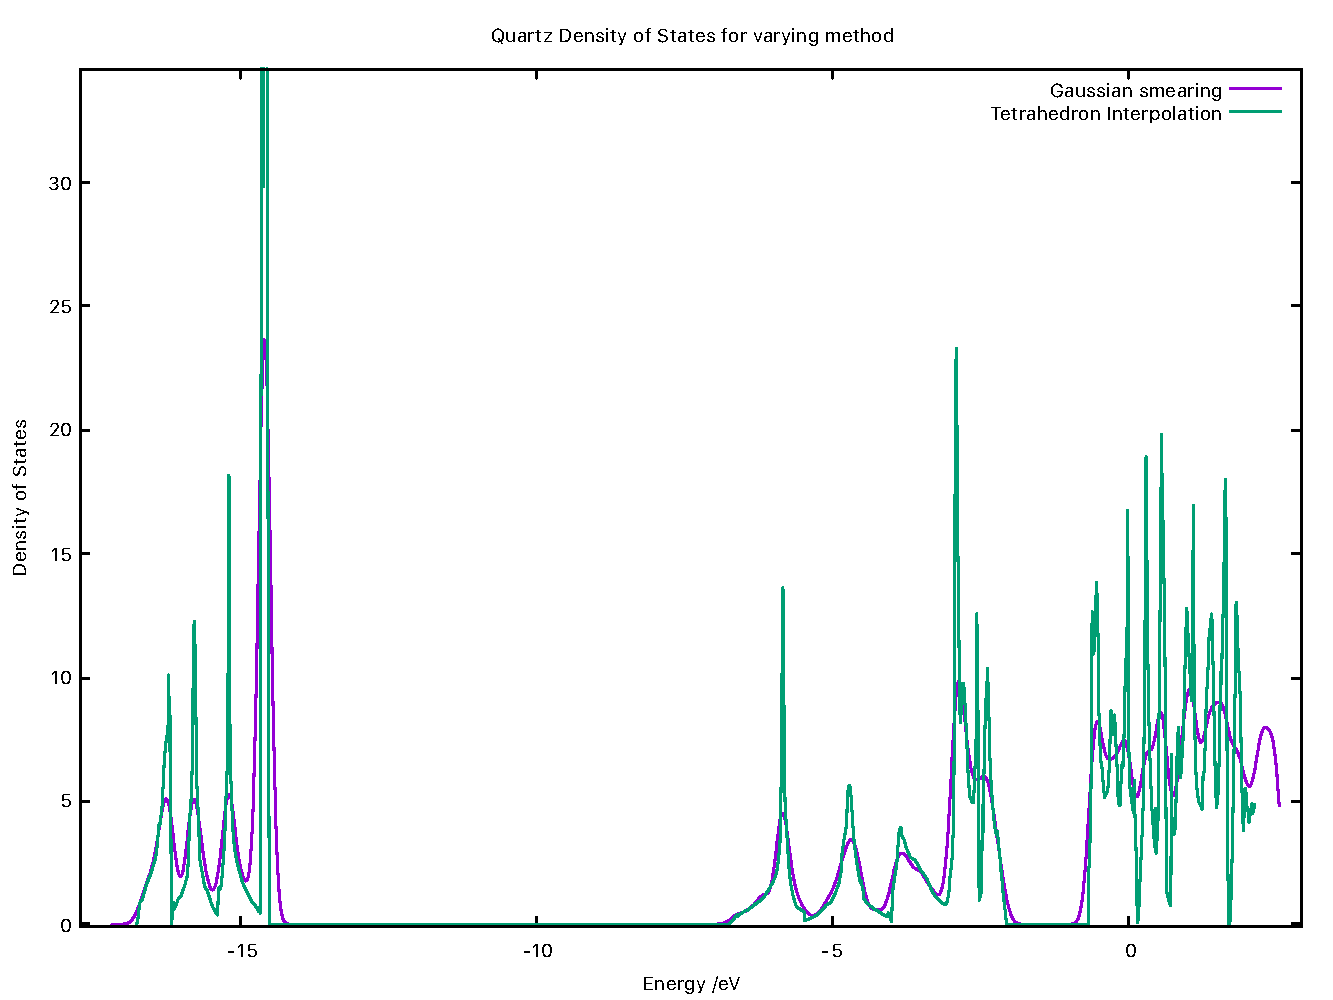
\includegraphics[width=8.2cm]{quartz-dos-data/quartz-method-dos.pdf}
		\subcaption{Here the Gaussian smearing value is 0.010,\\for both the k-point grid is (7 7 7)}
		\label{fig:quartz-method-dos}
	\end{subfigure}%
	\begin{subfigure}[t]{0.5\textwidth}
		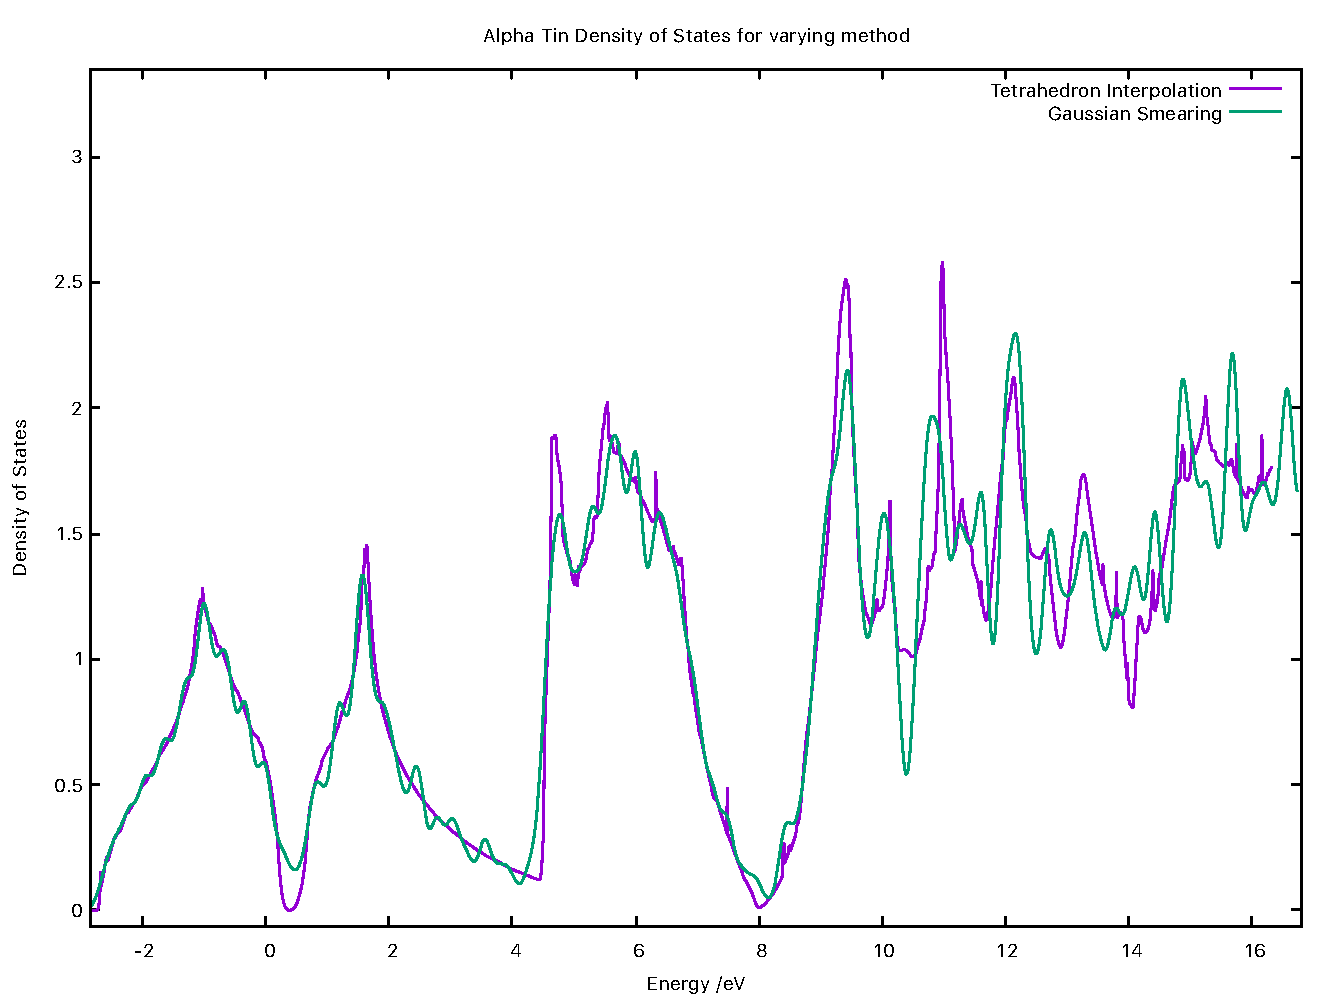
\includegraphics[width=8.2cm]{alpha-dos-data/alpha-method-dos.pdf}
		\subcaption{Here the Gaussian smearing value is 0.010, for both the k-point grid is (15 15 15)}
		\label{fig:alpha-method-dos}
	\end{subfigure}%
	\\
	\begin{subfigure}[t]{0.5\textwidth}
		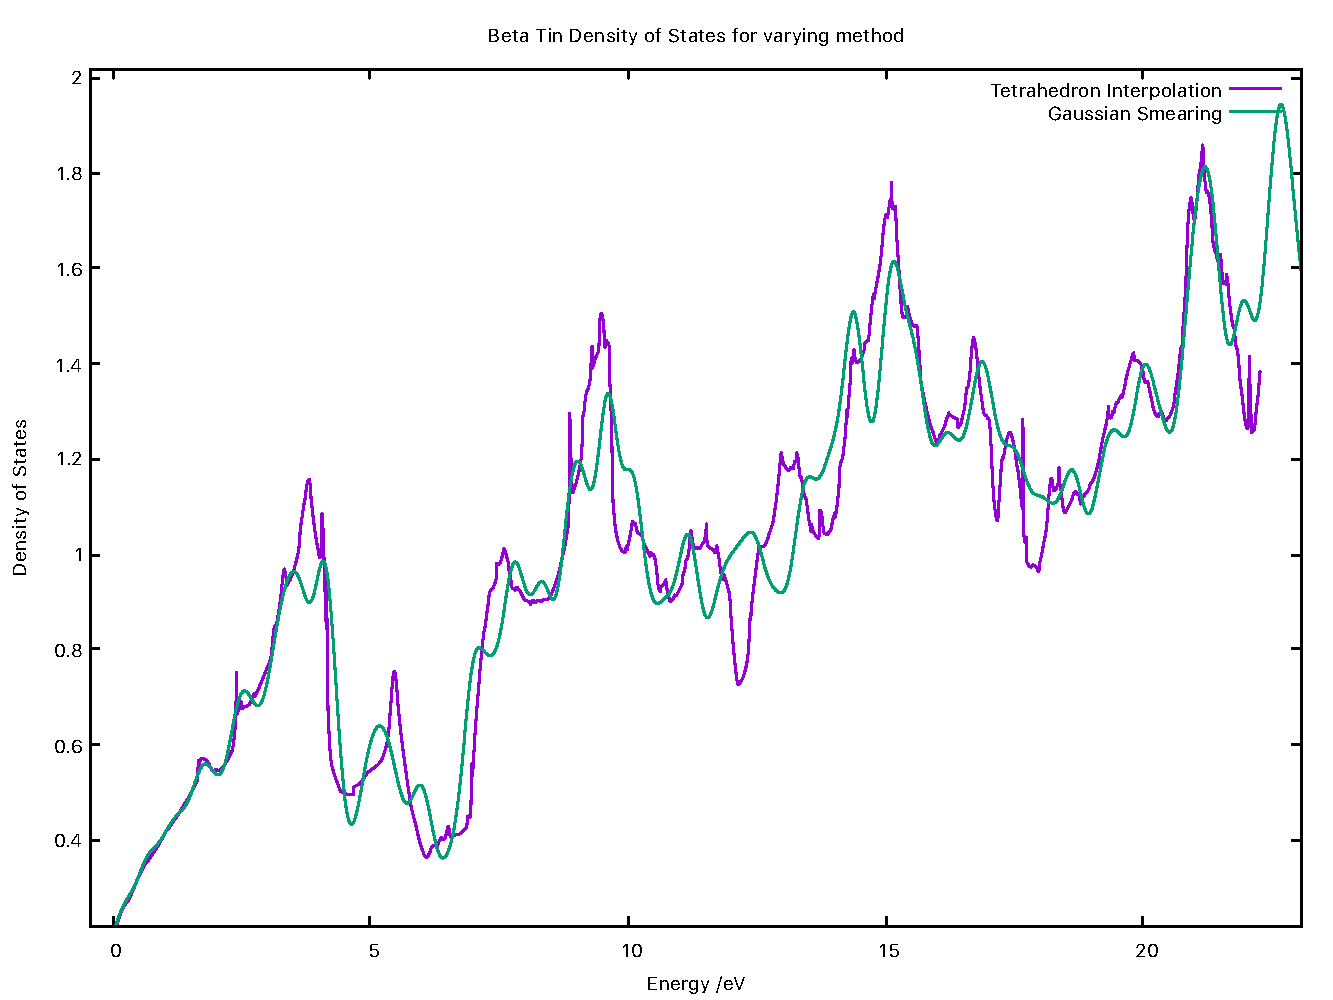
\includegraphics[width=8.2cm]{beta-dos-data/beta-method-dos.pdf}
		\subcaption{Here the Gaussian smearing value is 0.020, for both the k-point grid is (12 12 12)}
		\label{fig:beta-method-dos}
	\end{subfigure}
	\caption{The density fofstates plotted with Gaussian smearing and tetrahdron interpolation for Quartz (a), $\alpha$- (b) and $\beta$-tin (c).}
	\label{fig:m-vary}
\end{figure}

\bigskip

\noindent Based on these studies, optimal k-point grids and interpolation methods were chosen to plot the final density of states alongside the band structures as seen in Figure \ref{fig:banddos}. For quartz, Gaussian smearing was used with a value of 0.010 on a k-point grid of (7 7 7). This was quite computationally cheap and reached a level of convergence acceptable to study alongside the band structure. The tetrehedron method produced a far too noisy density of states that was hard to read. For $\alpha$-tin the tetrahderon method was chosen with a k-point grid of (15 15 15). This also prodcued the leats noisy results at an acceptable accuracy. One key thing to note is that the density of states is expected to reach zero at the Fermi level. This was not achieved with smearing but is with tetrahedron interpolation. Finally, $\beta$-quartz was plotted with a k-point grid of (12 12 12) with a smearing value of 0.020. This was significantly more computationally expensive than the other two, hence the higher smearing value. The density of states for the varying choices all followed a similar trend with roughly similar peaks and increasing as the energy increased but these chosen values provided the clearest result for an acceptable level of expense.

\begin{figure}[h!!!!!]
	\centering
	\begin{subfigure}[t]{0.5\textwidth}
		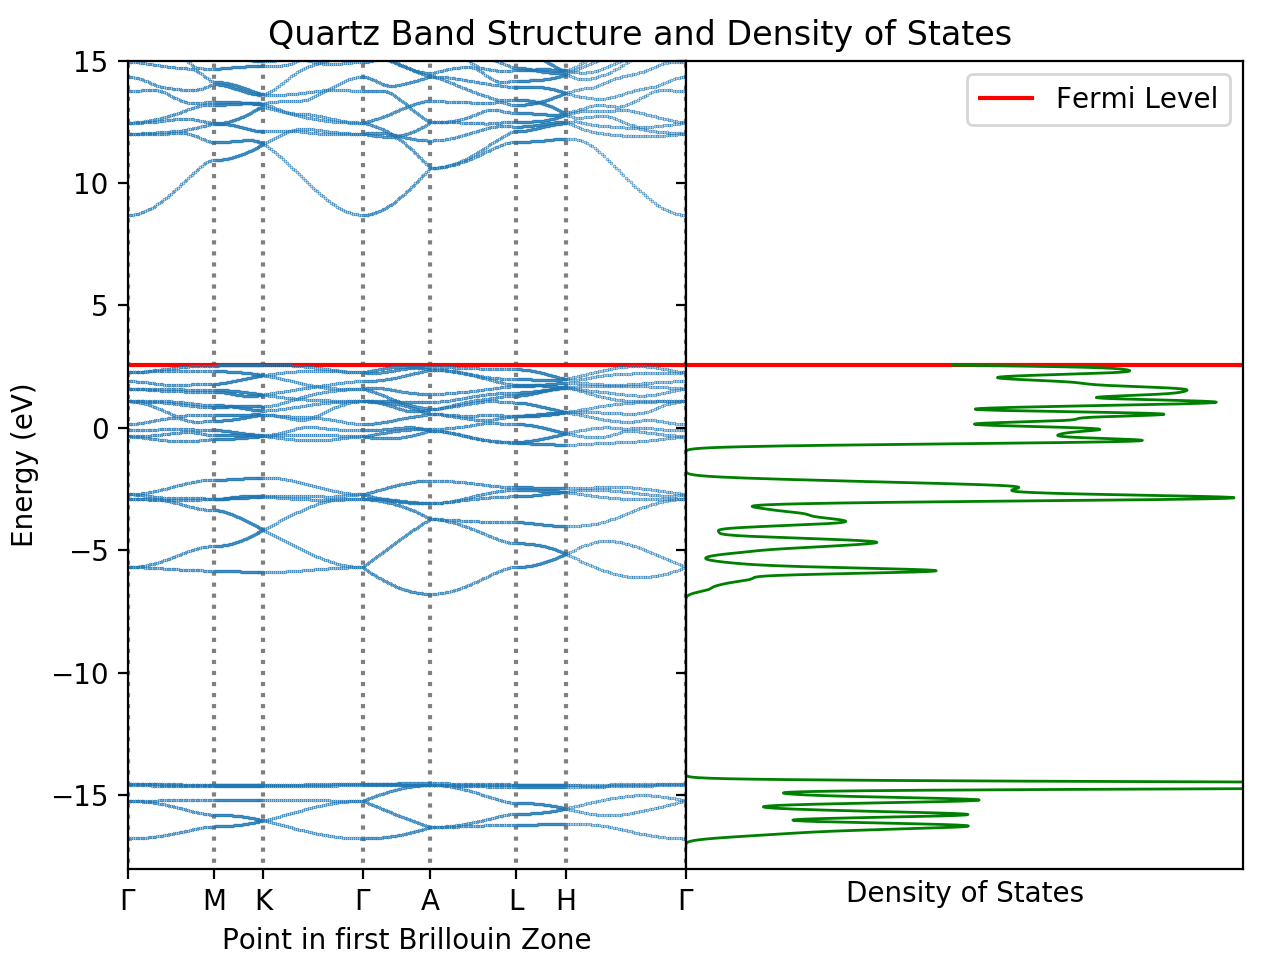
\includegraphics[width=8.2cm]{quartz-dos-data/quartz-band-dos.png}
		\subcaption{Note the large peak in the density of states\\at about 15 eV has been cut for clarity.}
		\label{fig:quartz-band-dos}
	\end{subfigure}%
	\begin{subfigure}[t]{0.5\textwidth}
		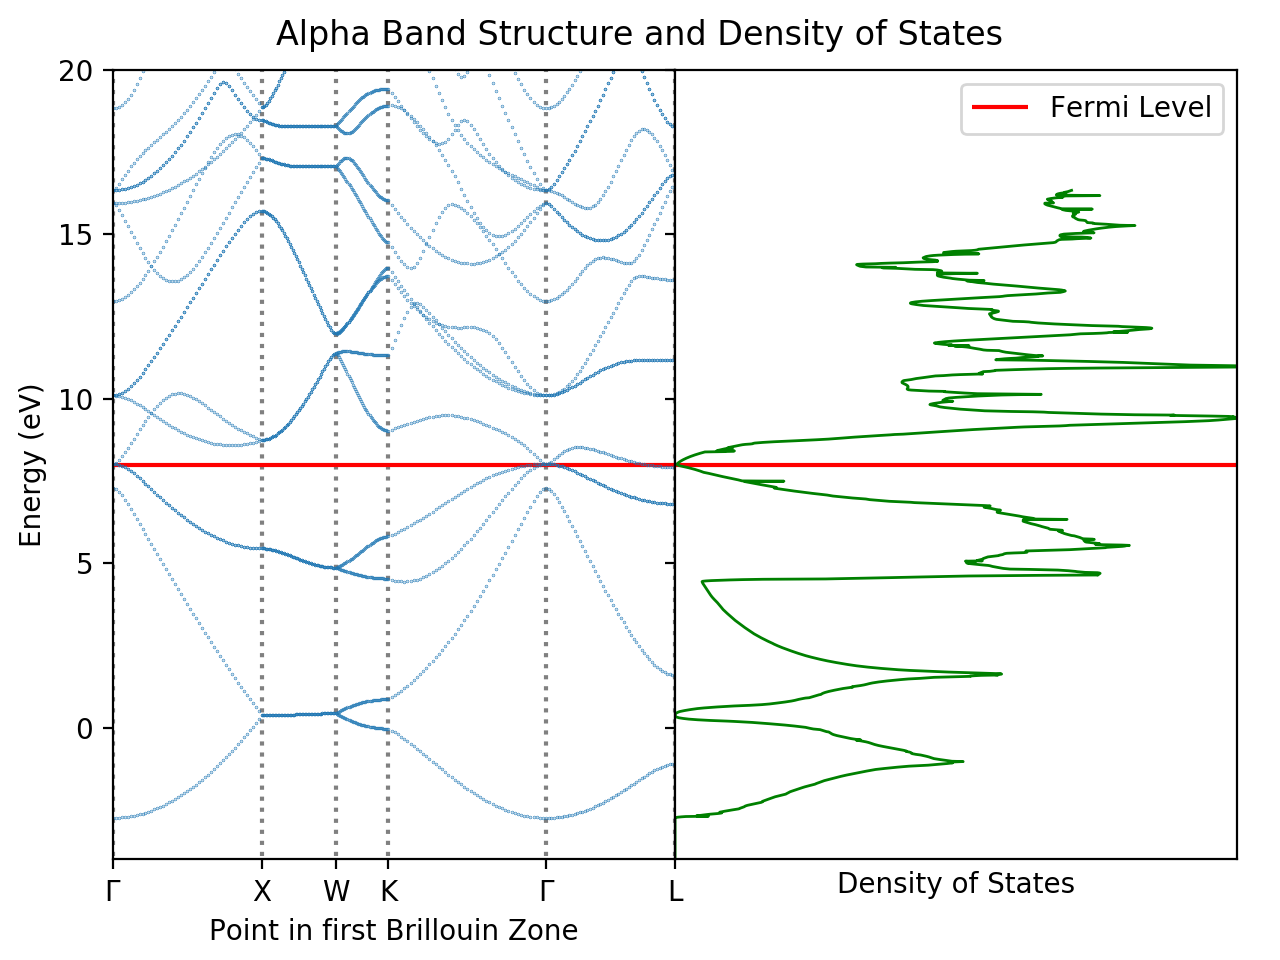
\includegraphics[width=8.2cm]{alpha-dos-data/alpha-bands-dos.png}
		\subcaption{Note that the central states producing a large peak at lower energies has been cut for clarity.}
		\label{fig:alpha-band-dos}
	\end{subfigure}%
	\\
	\begin{subfigure}[t]{0.5\textwidth}
		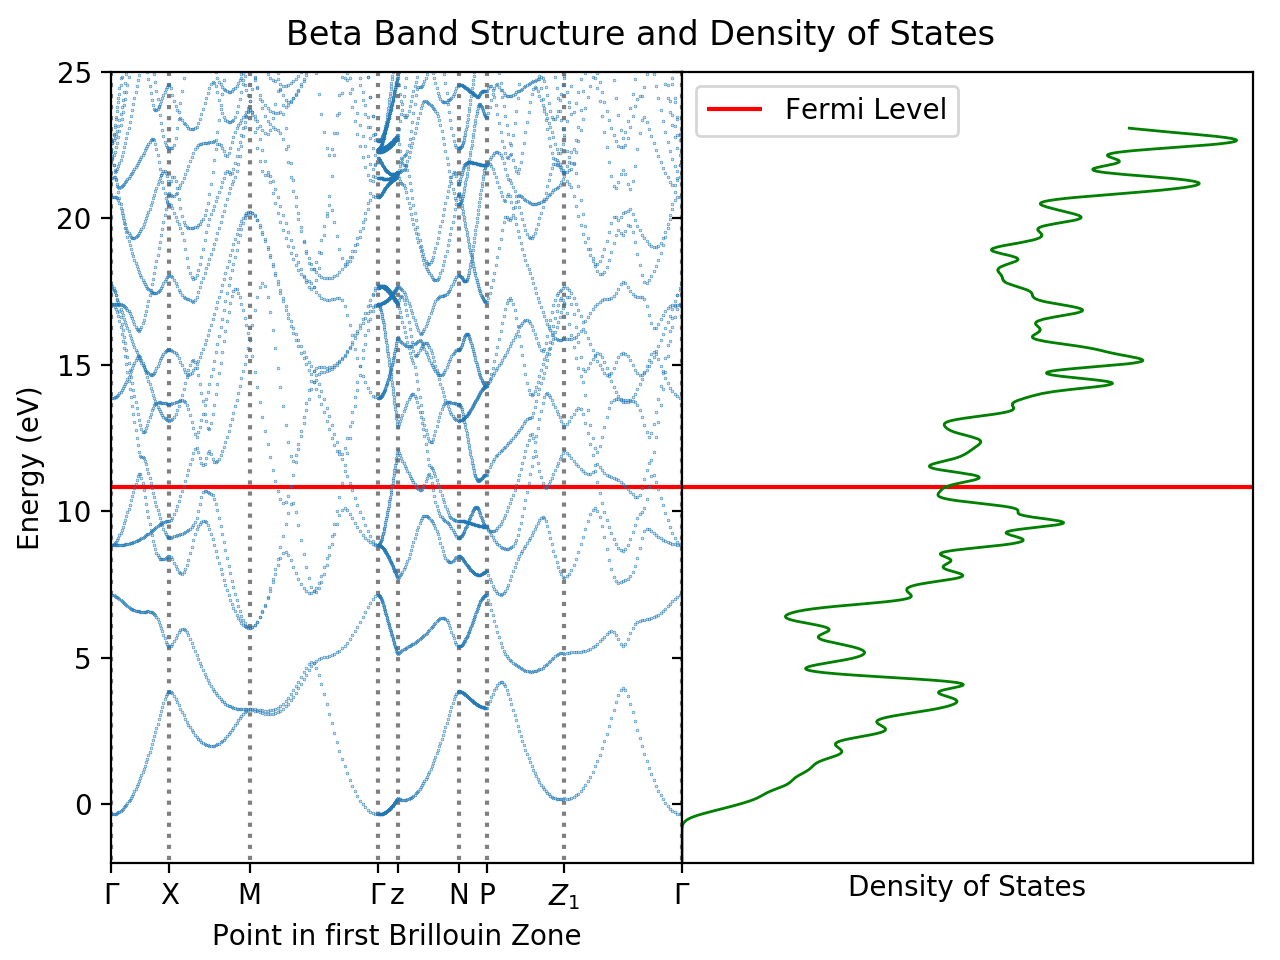
\includegraphics[width=8.2cm]{beta-dos-data/beta-bands-dos.png}
		\subcaption{Note that the central states producing a large peak at lower energies has been cut for clarity.}
		\label{fig:beta-band-dos}
	\end{subfigure}
	\caption{The band structures and density of states for Quartz, $\alpha$- and $\beta$-tin.}
	\label{fig:banddos}
\end{figure}

\bigskip

\noindent The final results for the density of states and band structures are shown in Figure \ref{fig:banddos}. The two plots agree well for all three systems. Quartz has a bandgap of roughly 6 eV. $\alpha$-tin has a zero band gap and is a semiconductor. $\beta$-tin has no bandgap and is a metal. The qualitiative results concur with the know properties of these structures. The quartz result agrees with other DFT studies\cite{qdft} but is significantly lower than the experimental result of 9.65 eV\cite{qexp}. However, DFT is commonly known to underestimate band gaps as is the case here. For $\alpha$-tin there have been some study into whether it is better classified as a semimetal\cite{asemi}. The results stated that under further study to confirm some criterion, that $alpha$-tin would be considered a zero band gap semiconductor.

\clearpage
\section*{Tin's Phases and Transitions}

Figure \ref{fig:sn-phase} shows the SCF energies for varying unit cell volumes of $\alpha$- and $\beta$-tin. They have both been fit with the Vinet equation of state and a common tangent between them. Using the Vinet fit, the $B_0$, $B_0^{\prime}$, equilibrium energy per atom and equilibrium volume per atom was found. The negative of the common tangent gradient provides the phase transition pressure and the volume collapse can be found be the change in volume at the common tangent points. All of these results are shown in Table \ref{tab:sn-phase}.

\begin{figure}[h!!!!!]
\centering
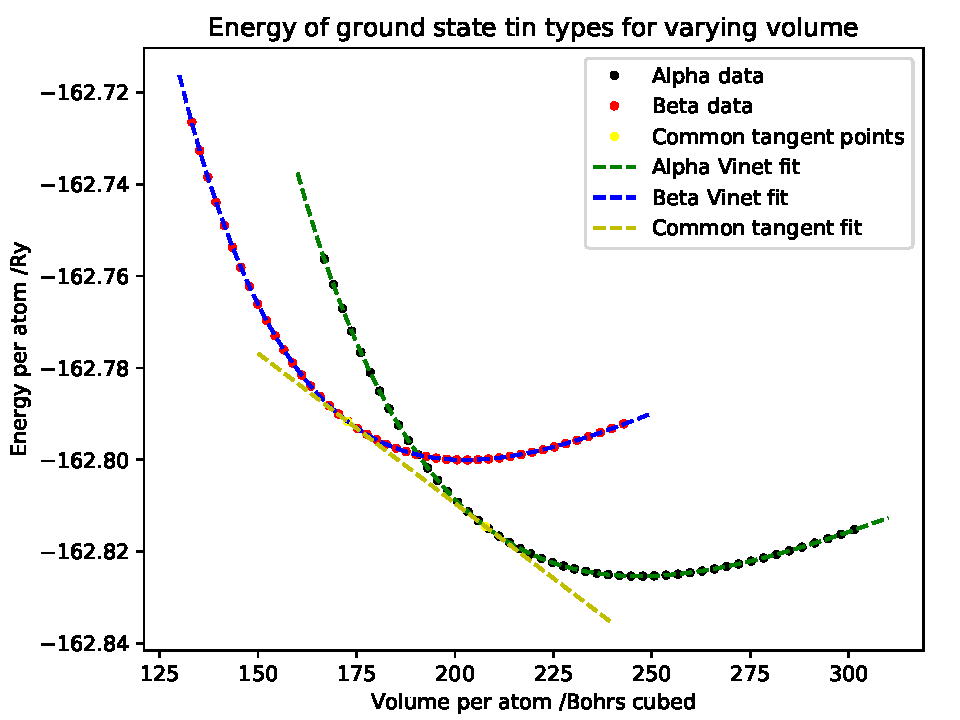
\includegraphics[width=12cm]{sn-phase-data/sn-phase.pdf}
\caption{The SCF energy per atom results for varying volumes per atom of $\alpha$- and $\beta$-tin with Vinet equation of state fits. A common tangent to these fits has also been produced.}
\label{fig:sn-phase}
\end{figure}

\begin{table}[h!!!!]
	\centering
\begin{tabular}{l|c|c|}
	\cline{2-3}
	\multicolumn{1}{c|}{}                                             & $\alpha$-tin          & $\beta$-tin          \\ \hline
	\multicolumn{1}{|l|}{$B_0$ (Error) /GPa}                          & 36.785 (0.105 \%)               & 41.049 (0.251 \%)              \\ \hline
	\multicolumn{1}{|l|}{$B_0^{\prime}$ (Error)}                    & 5.035 (0.171 \%)      & 4.914 (0.345 \%)     \\ \hline
	\multicolumn{1}{|l|}{Equilibrium Energy per atom (Error) /eV}       & -11.972 (\num{4.175e-6} \%)               & -11.971 (\num{8.081e-6} \%)    \\ \hline
	\multicolumn{1}{|l|}{Equilibrium Volume per atom (Error) /\AA$^3$}       & 35.559 (\num{6.446e-3} \%)       & 30.019     (0.014 \%)           \\ \hline
	\multicolumn{1}{|l|}{Transition Pressure (Error) /GPa}                   & \multicolumn{2}{c|}{9.603 (\num{6.315e-10} \%)}                   \\ \hline
	\multicolumn{1}{|l|}{Volume Collapse at Transition Pressure (\%)} & \multicolumn{2}{c|}{20.359}                  \\ \hline
\end{tabular}
\caption{The results from the fitting the Vinet equation of state to each of the $\alpha$- and $\beta$-tin data sets and then a linear fit for a common tangent.}
\label{tab:sn-phase}
\end{table}

\noindent This set of data compares well to other DFT results, such as the results at Materials Project for $\alpha$- and $\beta$-tin. Here the bulk modulus is determined to be 38 GPa\footnote{https://materialsproject.org/materials/mp-117/} and 46 GPa\footnote{https://materialsproject.org/materials/mp-84/} for $\alpha$ and $\beta$ respectively, which is in good agreement with the fit results from this experiment. They also achieve a similar volume per atom with the Vinet equation of state at 36.838 \AA$^3$ and 28.402 \AA$^3$ respectively. This lends support that the results from the DFT calculations and the analysis is done correctly but does not mean that the results are representitive of true experimental data.

\bigskip

\noindent When compared to experimental data there are noticeable differences. The bulk moduli  of $\alpha$- and $\beta$-tin have been found as 53 GPa\cite{PRICE} and 58.2 GPa\cite{smithells} respectively. There is a noticeable difference in these values from the ones gathered by the fits in this report. However, due to the consistency with other DFT results this is likely due to the DFT methods applied here or DFT itself creating the discrepancy.

\bigskip

\noindent The transition pressure agrees well with other experimental results. The phase diagram of tin\cite{pt} shows a rough extrapolation of the transition of $\alpha$- and $\beta$-tin to zero pressure at just over 10 GPa (the value is stated as roughly 10 GPa and 50K) which is in good agreement with the derived result. The volume change at the transition is also consistent with experimental results of about 20\%\cite{jerry}(This source also achieves a similar volume per atom for $\alpha$-tin). However, other attempts at calculating the transition pressure and temperature of $\alpha$- and $\beta$-tin have found different results\cite{firstprinc}. Here a frozen phonon approach was taken to get the phonon density of states, which wa sthen used to calculate various thermodynamic constants. This study found that at zero Kelvin the transition pressure was roughly 0.3 GPa, and qutoes other studies finding between 0.2-0.8 GPa, although all are theoretical studies. Clearly there is issues in accurately studying tin not only in GGA DFT as used here, but in other approaches as well. This is likely due to more complex structure of $\beta$-tin and particularly phase transitions in general.

\clearpage
\printbibliography
	
\end{document}